%%%%%%
%BASE
%%%
\documentclass[12pt,a4paper]{article}
\usepackage[utf8]{inputenc}
\usepackage[T1]{fontenc}
\usepackage[francais]{babel}
\usepackage{graphicx}
\usepackage{frcursive}

%%%%%
%MATHS
%%%
\usepackage{amsmath}
\usepackage{array}
\usepackage{multicol}

%%%%%
%COULEURS
%%%
\usepackage{xcolor}
\usepackage{color}

%%%%%
%PUCES
%%%
\usepackage{pifont}

\everymath{\displaystyle}
\usepackage{hyperref}
\setlength{\parindent}{10px}



%%%%%
%Haut de Page
%%%
\usepackage{fancybox}
\usepackage{fancyhdr}
\usepackage[left=1.3cm,right=1.2cm,top=2cm,bottom=1.5cm]{geometry}
\pagestyle{fancy}
\fancyhead[L]{Lespinasse Florentin}
\fancyhead[C]{}
\fancyhead[R]{1STI2D4~~~~~~~~\today}

\begin{document}
\begin{cursive}
\begin{center}
        \shadowbox{\begin{large}
                \textcolor{black}{\'Emile Zola}
        \end{large}}
    \end{center}
    \vspace{0.5 cm}
\setlength{\columnseprule}{0.25pt}
\begin{multicols}{2}
\ding{99} Nom complet,
\vspace{0.1 cm} \\ 
\'Emile \'Edouard Charles Antoine Zola\par
\ding{99} Aussi appelé \textit{Le Maître de Médan}\par
\ding{99} Est né le $2~Avril~1840$ à Paris \par
\ding{99} Mort le $29~septembre~1902$ à Paris\par
\ding{99} De Nationalité Fran\c caise\par
\centering

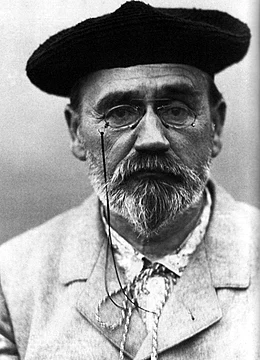
\includegraphics[scale=0.5]{Emile_Zola.png}
\end{multicols}
\dotfill
\begin{center}
\ding{72} \'Etudes\par
\end{center}

\ding{99} Après 2 tentative, le Bac rest un echec pour lui. L'université lui est inderdite après cela.\par
\ding{99} Il vit dans la pauvreté avec sa mère à charge. Son père est mort d'une pneumonie quand l'auteur avait 7ans.\par
\ding{99} Zola trouve du travail aux écrits à la Docks de Paris en 1840 mais cela ne lui pla\^it pas, il démissione 2 mois après.\par
\ding{99} Il est engagé par Louis Hachette comme commis. Il y apprends beaucoup de choses, et décide pendant ses loisirs, de travailler avec acharnement sur un livre qui sera publié, \textit{ Les Contes à Ninon (en 1864)}\par
\ding{99} \'Emile Zola, écrit des nouvelles, des romans, des pièces de théâtre et des poèmes.\par
\ding{99} Mais est aussi un journaliste politique. Le 13 janvier 1898, il publie dans le Figaro un article \textit{J'acuses...!} pour dénoncer l'affaire Dreyfus.\par
\ding{99} Zola meurs dans son lit à cause d'une combustion lente de la cheminée de sa chambre. \par

\begin{center}
\ding{72} O\oe uvres \par
\end{center}


\ding{99} \textit{Les Contes à Ninon} son premier ouvrage, en 1864\par
\ding{99} Son premier roman, \textit{La Confession de Claude} en 1865\par
\ding{99} \textit{Germinal} en 1885\par

\end{cursive}
\end{document}

